%!TEX root=../GaugeCNNTheory.tex


\section{اشتراک وزن مستقل از مختصات و کرنل‌های $G$-راهبری‌پذیر}
\label{apx:coord_indep_weight_sharing}


\begin{figure}
    \centering
    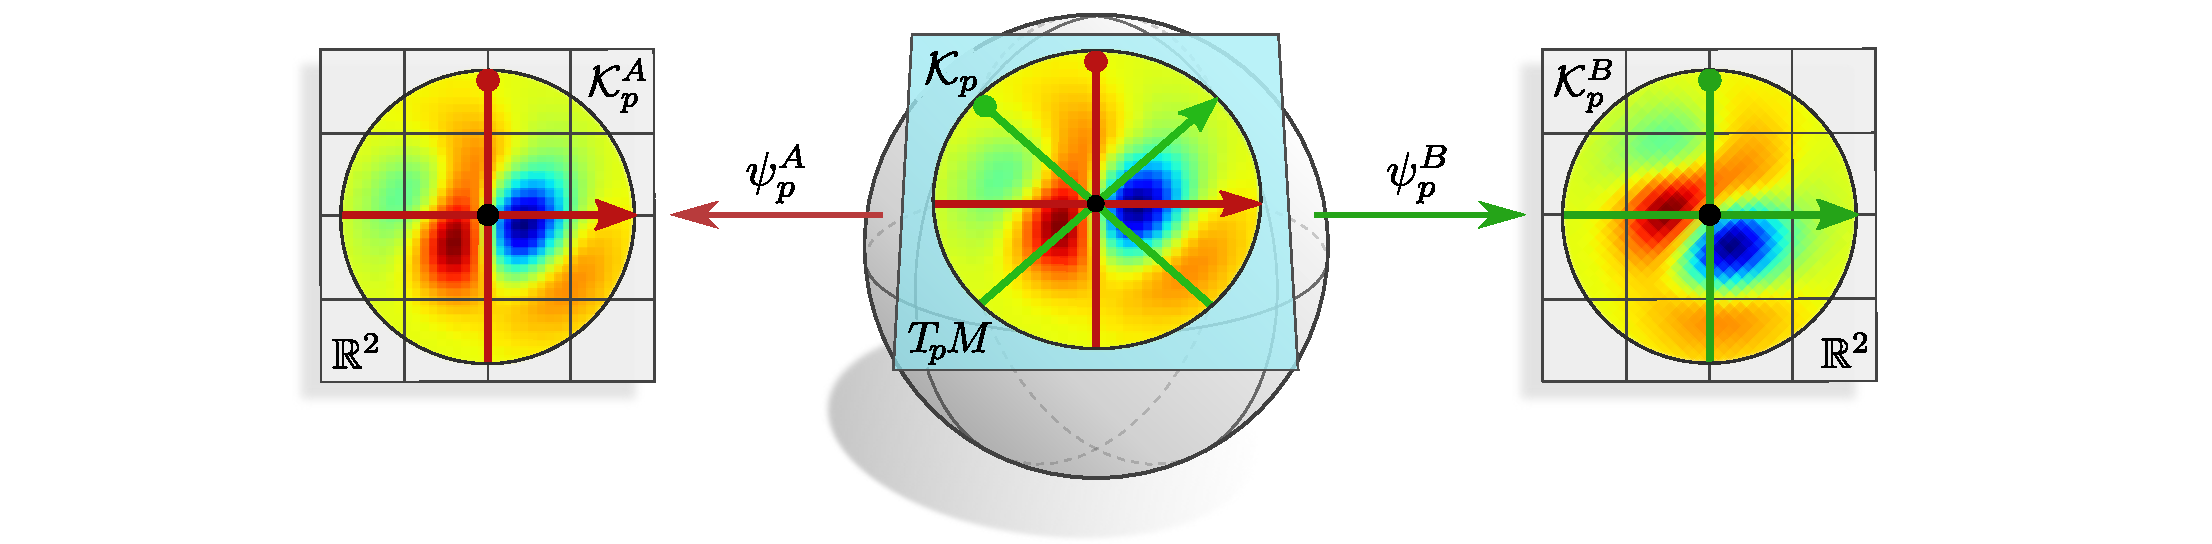
\includegraphics[width=1.\columnwidth]{figures/kernel_apx_coordinatization.pdf}
    \vspace*{-3.5ex}
    \caption{\small
        یک کرنل مستقل از مختصات \emph{داده شده} $\Kp$ روی فضای مماس $\TpM$ ممکن است در پیمانه‌های دلخواه $\psi_p^A$ یا $\psi_p^B$ نمایش داده شود.
        عبارات مختصاتی آن $\Kp^A$ و $\Kp^B$ روی $\R^d$ به طور کلی با یکدیگر متفاوت هستند.
        کرنل‌های $G$-راهبری‌پذیر این ویژگی را دارند که دقیقاً شکل یکسانی را در تمام پیمانه‌ها به خود می‌گیرند، یعنی در $\Kp^A = \Kp^B = K$ صدق می‌کنند (در تصویر نشان داده نشده است).
    }
    \label{fig:kernel_apx_coordinatization}
\end{figure}


\begin{figure}
    \centering
    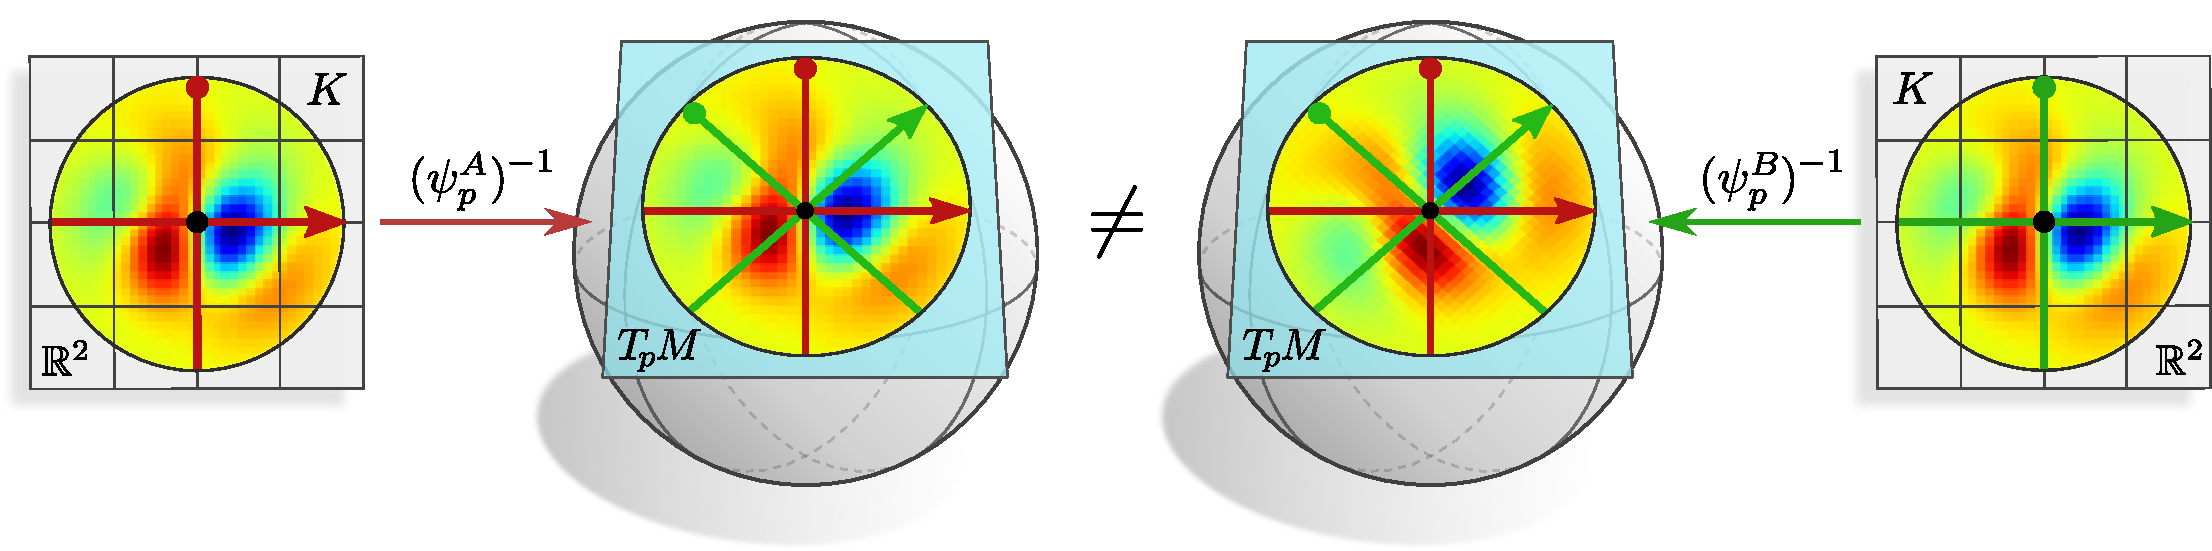
\includegraphics[width=1.\columnwidth]{figures/kernel_apx_sharing.pdf}
    \vspace*{-3.5ex}
    \caption{\small
        یک کرنل مستقل از مختصات ممکن است با \emph{اشتراک‌گذاری} یک کرنل داده شده $K$ روی $\R^d$ نسبت به یک چارچوب مرجع \emph{تعریف شود}.
        انتخاب‌های مختلف از چارچوب‌ها منجر به یک کرنل مستقل از مختصات متفاوت می‌شود.
        کرنل‌های $G$-راهبری‌پذیر این ویژگی را دارند که دقیقاً همان کرنل مستقل از مختصات را تولید می‌کنند، مستقل از چارچوب مرجع انتخاب شده که در امتداد آن به اشتراک گذاشته می‌شوند (در تصویر نشان داده نشده است).
        این امر امکان اشتراک وزن مستقل از مختصات را فراهم می‌کند.
    }
    \label{fig:kernel_apx_sharing}
\end{figure}


یک فرض اساسی در طراحی کانولوشن‌های $\GM$ این است که کرنل‌های $K$ روی $\R^d$ نسبت به یک انتخاب از چارچوب مرجع، همانطور که در شکل~\ref{fig:kernel_apx_sharing} به تصویر کشیده شده است، به اشتراک گذاشته می‌شوند.
برای کرنل‌های عمومی، انتخاب‌های مختلف از چارچوب‌ها منجر به ترازهای متفاوتی از کرنل مستقل از مختصات حاصل روی فضای مماس~$\TpM$ می‌شود
-- بنابراین فرآیند اشتراک وزن، مستقل از مختصات نیست.
شکل~\ref{fig:kernel_apx_coordinatization} وضعیت متفاوتی را نشان می‌دهد:
در اینجا ما یک کرنل مستقل از مختصات $\Kp$ را فرض می‌کنیم که از قبل روی~$\TpM$ داده شده است و آن را در پیمانه‌های مختلف روی~$\R^d$ بیان می‌کنیم.
نمایش‌های مختصاتی $\Kp^A$ و $\Kp^B$ به طور کلی با یکدیگر موافق نیستند اما ساختار، مستقل از مختصات است.


کرنل‌های $G$-راهبری‌پذیر دقیقاً به گونه‌ای محدود شده‌اند که استقلال از مختصات فرآیند اشتراک وزن را تضمین کنند.
اشتراک‌گذاری آنها نسبت به چارچوب‌های مختلف منجر به همان کرنل مستقل از مختصات روی فضای مماس می‌شود،
یعنی هیچ تفاوتی بین دو کرنل در وسط شکل~\ref{fig:kernel_apx_sharing} وجود نخواهد داشت.
به طور معادل، کرنل مستقل از مختصات حاصل روی $\TpM$ هنگام بیان در پیمانه‌های مختلف، شکل یکسانی $\Kp^A = \Kp^B = K$ را به خود می‌گیرد،
یعنی کرنل چپ و راست در شکل~\ref{fig:kernel_apx_coordinatization} با هم موافق خواهند بود.


توجه داشته باشید که این لزوماً به این معنا نیست که کرنل به معنای $K(g\mathscr{v}) = K(\mathscr{v})$ برای هر $g\in G$ و هر~$\mathscr{v}\in\R^d$ ناوردا باشد، همانطور که شهود بصری ممکن است القا کند.
این در واقع یک مورد خاص برای کرنل‌هایی است که بین میدان‌های اسکالر نگاشت انجام می‌دهند، یعنی برای آنهایی که هم $\rhoin$ و هم $\rhoout$ نمایش‌های بدیهی هستند (به عنوان مثال شکل~\ref{fig:intro_steerable_kernel} برای $G=\Flip$ یا شکل~\ref{fig:zonal_kernel} برای $G=\O2$ را ببینید).
برای انواع میدان عمومی‌تر، کرنل‌ها باید هموردای پیمانه باشند، یعنی باید محدودیت $G$-راهبری‌پذیری
$K(g\mkern1.5mu \mathscr{v}) = \detg^{-1} \rhoout(g)\: K(\mathscr{v})\: \rhoin(g)^{-1}$
را برآورده کنند که امکان هدایت کانال‌های کرنل ${\cout\times\cin}$ را فراهم می‌کند (در تصویر نشان داده نشده است).
البته، کرنل‌های $G$-راهبری‌پذیر را می‌توان به معنای \emph{ناوردای} پیمانه تفسیر کرد به این معنا که
$K(\mathscr{v}) = \detg \rhoout(g)^{-1}\: K(g\mkern1.5mu \mathscr{v})\: \rhoin(g)$
برای هر $g\in G$ و هر~$\mathscr{v}\in\R^d$.
این مفهوم از ناوردایی پیمانه، اشتراک مستقل از مختصات کرنل‌های $G$-راهبری‌پذیر را ممکن می‌سازد.


یک بحث دقیق‌تر در مورد کرنل‌های مستقل از مختصات و عبارات مختصاتی آنها در بخش~\ref{sec:kernel_field_trafos} یافت می‌شود.
محدودیت $G$-راهبری‌پذیری در بخش~\ref{sec:gauge_conv} استخراج شده است.